\documentclass[11pt,a4paper]{article}
\usepackage[utf8]{inputenc}
\usepackage[left=2cm,text={17cm, 24cm},top=3cm]{geometry}
\usepackage{times}
\usepackage[czech]{babel}
\usepackage[T1]{fontenc}

\author{Alena Tesařová}
\usepackage[ruled,czech,linesnumbered,longend,noline]{algorithm2e}
\usepackage{graphics}
\usepackage{float}

\DeclareGraphicsExtensions{.png,.pdf}
\usepackage{hyperref}
\usepackage{cprotect}
\usepackage{graphicx}

\usepackage{pdflscape}
\usepackage{multirow}

\begin{document}

\begin{titlepage}

\begin{center}
\Huge
\textsc{Fakulta informačních technologií\\
Vysoké učení technické v~Brně}\\
\vspace{\stretch{0.382}}
\Huge Implementace překladače imperativního jazyka IFJ17
\\
\medskip
{\Large Tým 016 - varianta II}
\vspace{\stretch{0.618}}
\end{center}


\begin{LARGE}
\noindent
\textbf{ Řešitelé a rozdělení bodů } \\ \\
\end{LARGE}
{\Large 
Alena Tesařová (xtesar36) : 25 \% -- vedoucí\\
Jan Šorm (xsormj00) : 25 \% \\
Daniel Uhříček (xuhric00) : 25 \% \\
Peter Uhrín (xuhrin02) : 25 \% 
}
\hfill
\today
\end{titlepage}



\section{Úvod}
Měli jsme za úkol implementovat překladač jazyka IFJ17, který je založený na jazyku BASIC. Zvolili jsme si variantu implementace tabulky symbolů pomocí tabulky s roptýlenými položkami. Soustředili jsme se na splnění základní funkčnosti programu, proto jsme neimplemetovali žádná rozšíření.

\section{Lexikální analýza}
Lexikální analyzátor (soubory\ \verb|lex.h| a \verb|lex.c|) je část překladače starající se o~rozeznávání a kategorizaci jednotlivých lexémů ze vstupního souboru s~programem a vrací token s~typem lexému, popřípadě s~řetězcem, obsahující dodatečná data. Náš lexikální analyzátor je implementovaný jako konečný stavový automat, jehož schéma je přiloženo výše. Jeho prvotní forma vypadala trochu jinak a samotný návrh stavového automatu se v~malých obměnách vyvíjel spolu s~implementací.

Diagram, který je zde uveden jako finální, reprezentuje současné fungování lexikálního analyzátoru, ale v~rámci zjednodušení implementace, popřípadě zefektivnění programu nebyly některé ze stavů z~diagramu implementovány jako samostatné stavy, ale byly včleněny do stavů jiných.

Kupříkladu kontrolování escape sekvence uvnitř řetězcových litérálů je v~diagramu zaznačeno pomocí více stavů (\verb|s_literal_esc|, \verb|s_literal_ord_1|, \verb|s_literal_ord_l|), ale kvůli zjednodušení a zefektivnění implementováno uvnitř stavu \verb|s_literal|.

Podobná situace je i u~stavu \verb|t_invalid|, který se v~diagramu vyskytuje třikrát. Jedná se o~tentýž stav, který byl však kvůli zpřehlednění diagramu použit na více místech.

Následuje popis použitých datových struktur a funkcí v~souborech\ \verb|token.h, lex.h, lex.c|.

\subsection{token.h}

\subsubsection*{Konstanty}

\cprotect\textbf{\verb|TOKEN_TYPE_NUM|} -- počet typů tokenu ve výčtu \verb|token_type_t|

\subsubsection*{Datové struktury}
\cprotect\textbf{\verb|token_type_t|}  -- výčtový typ uchovávající v~sobě typy, kterých může token nabývat \\ \\
\noindent
\cprotect\textbf{\verb|token_t|}  -- struktura tokenu, který je výstupem lexikálního analyzátoru a obsahuje v~sobě proměnnou \verb|type| typu \verb|token_type_t| uchovávající typ tokenu a proměnnou \verb|data| typu \verb|*char| ve které je uložen ukazatel na řetězec (řetězcový literál, číselný literál, nebo jméno identifikátoru) 

\subsection{lex.h}
\subsubsection*{Konstanty}

\cprotect\textbf{\verb|KEYWORDS_NUM|} -- počet klíčových a rezervovaných slov jazyka IFJ2017

\subsubsection*{Datové struktury}
\cprotect\textbf{\verb|state_t |} -- výčtový typ uchovávající stavy pro konečný stavový automat

\subsection{lex.c}
\subsubsection*{Datové struktury a důležité proměnné}

\cprotect\textbf{\verb|keywords|} -- pole retězců korespondujicích s~klíčovými a rezervovanými slovy jazyka IFJ2017 \\

\noindent
\cprotect\textbf{\verb|keywords_tokens|} -- pole typů tokenů korespondujících s~klíčovými a rezervovanými slovy jazyka IFJ2017 \\

\noindent
\cprotect\textbf{\verb|fr_source|} -- proměnná, která uchovává ukazatel na vstupní proud (otevřený soubor, nebo stdin)

\subsubsection*{Funkce}
\cprotect\textbf{\verb|file_init|} -- přiřadí ukazatel na otevřený vstupní proud do proměnné \verb|fr_source| \\ 

\noindent
\cprotect\textbf{\verb|edit_token|} -- funkce, která upraví typ a data struktury tokenu \\ 

\noindent
\cprotect\textbf{\verb|get_token|} -- hlavní funkce lexikálního analyzátoru, která při každém volání nalezne a kategorizuje následující lexém ve vstupním proudu a vrátí korespondující token

\begin{figure}[H]
	
	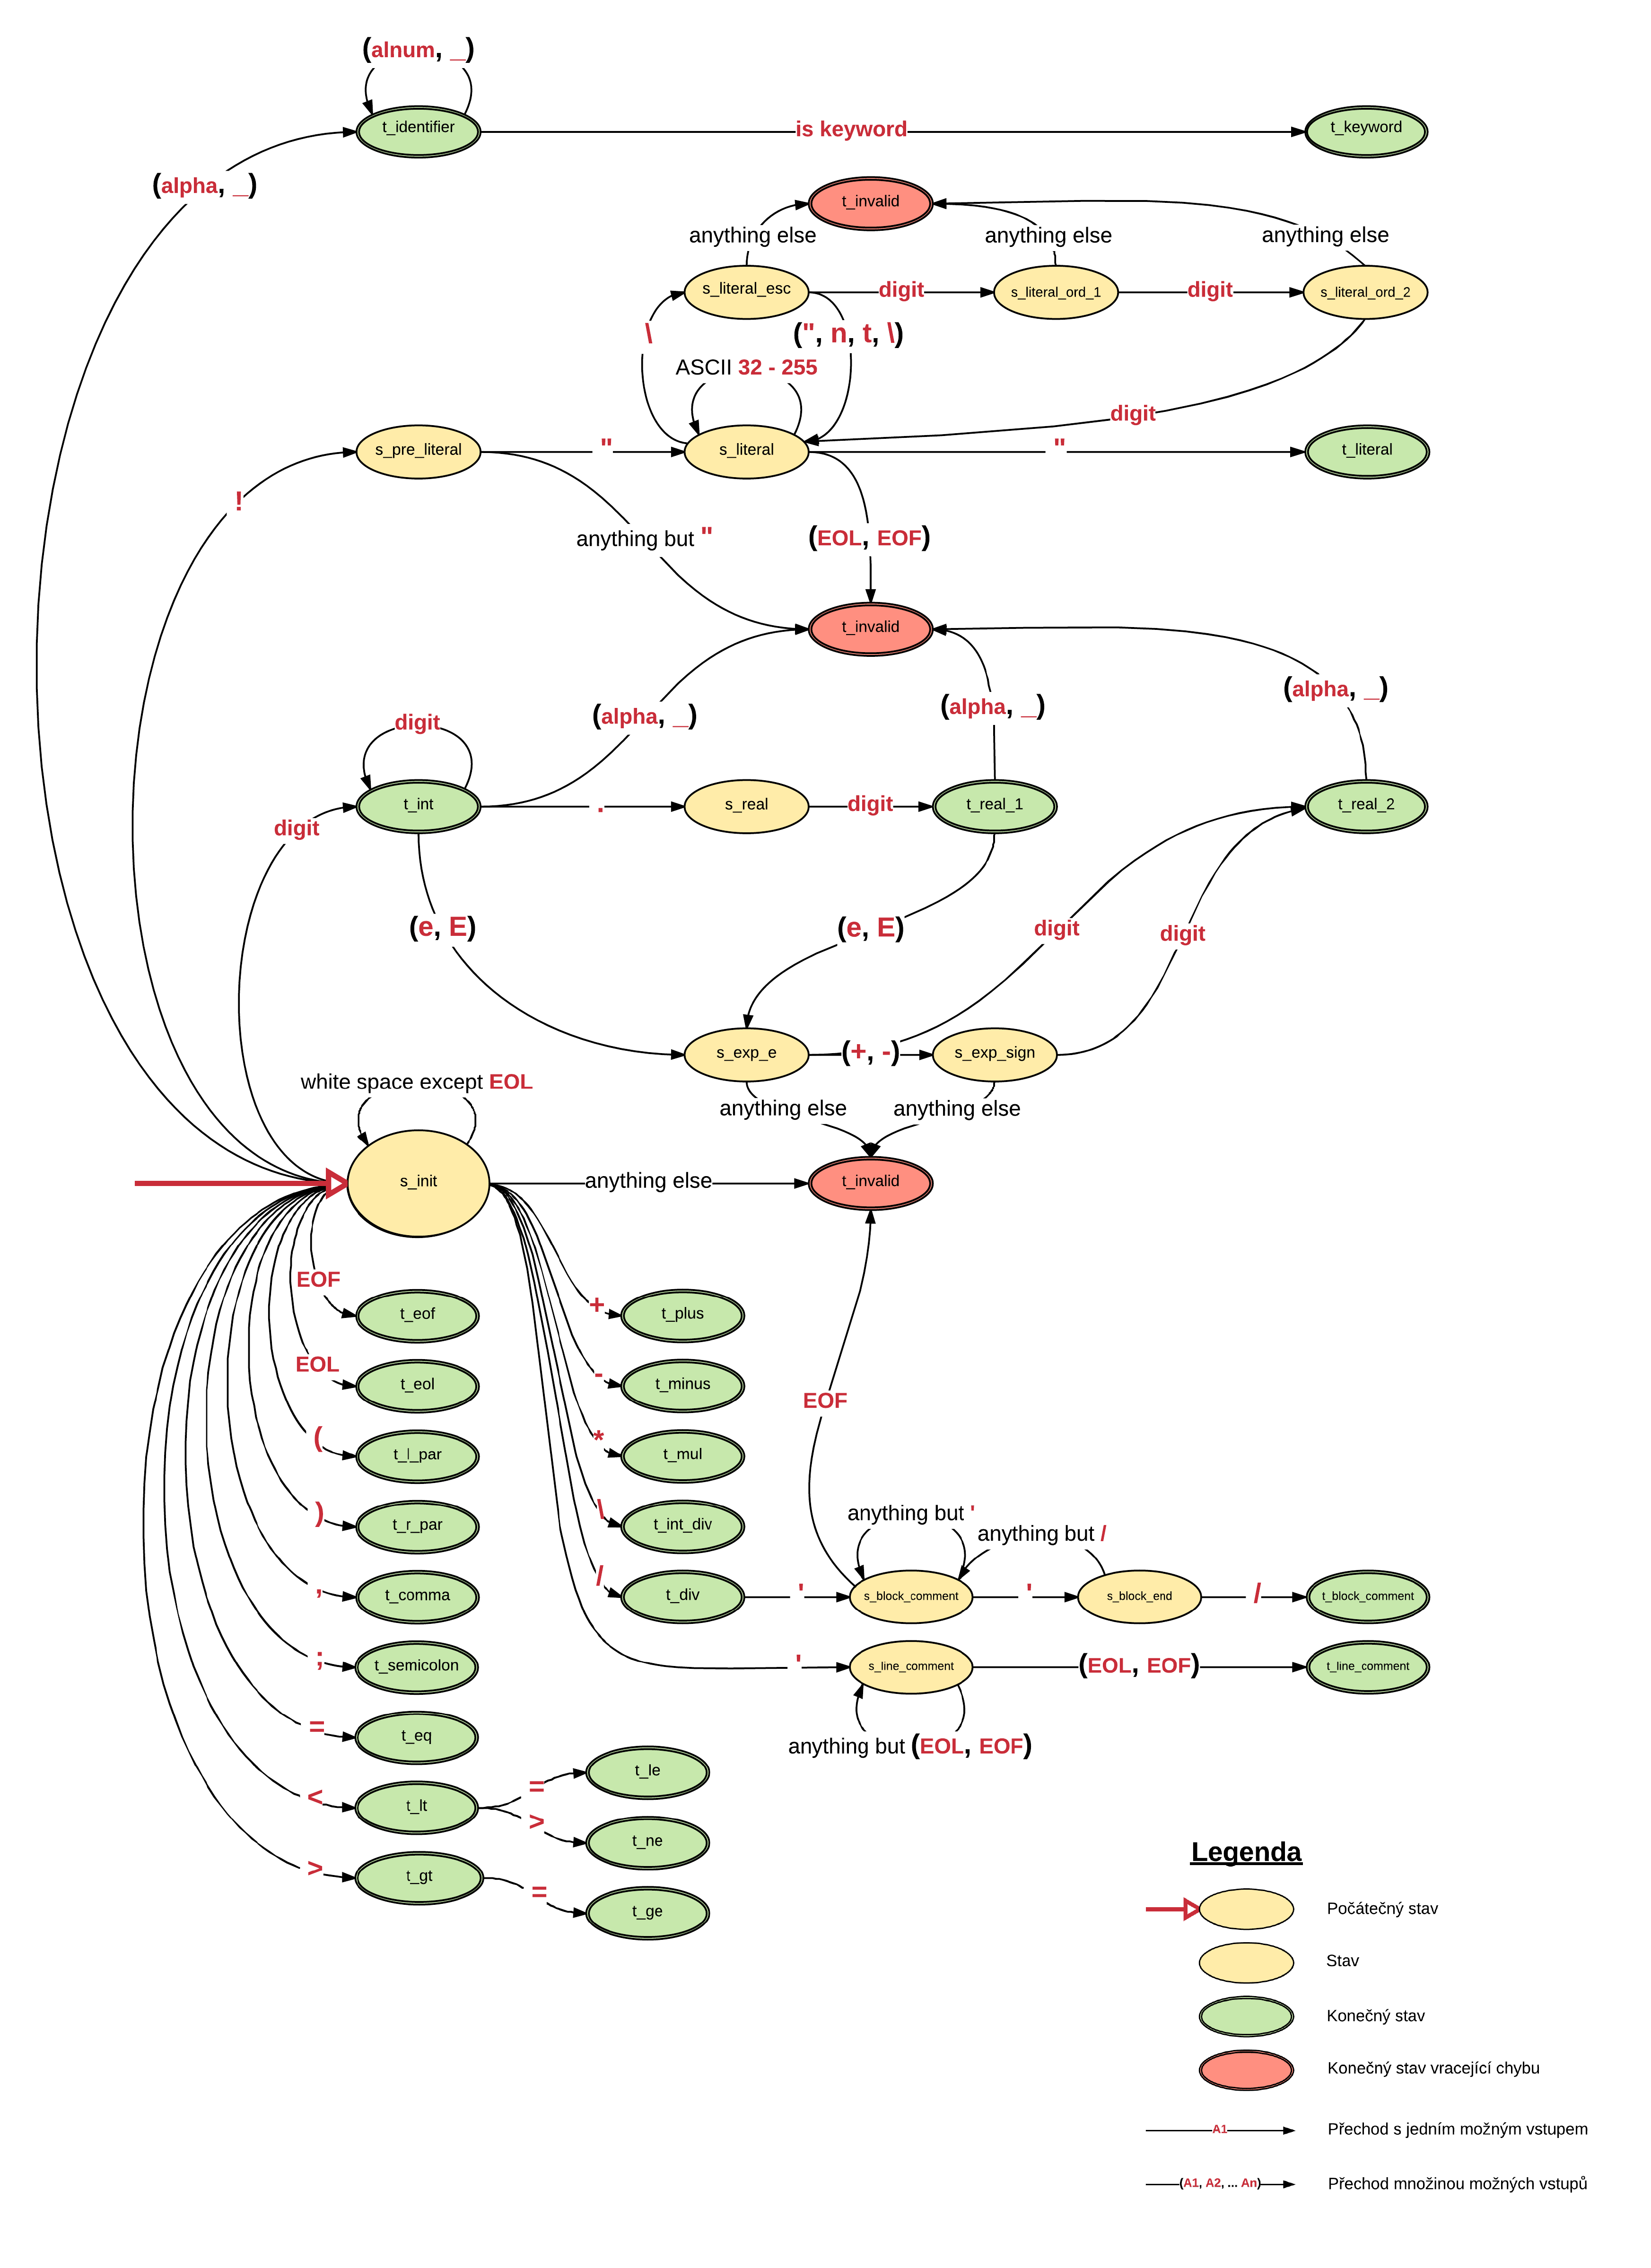
\includegraphics[width=17cm]{png/FSM_diagram.png} 
	\caption{Stavový automat pro lexikální analýzu}

\end{figure}



\section{Syntaktická analýza}
Syntaktický analyzátor (soubory \verb|parser.h|, \verb|parser.c|, \verb|expression.h|, \verb|expression.c|) je část překladače starající se o~syntaktickou kontrolu překládaného programu. V~našem případě je implementovaný metodou rekurzivního sestupu (v~souboru \verb|parser.c|) a precedenční analýzou výrazu (v~souboru \verb|expression.c|). Syntaktický analyzátor zároveň řídí celý běh překladu. Volá se z~něj lexikální analyzátor, ze kterého dostává tokeny, které následně zpracovává. Volá také funkce pro sémantickou analýzu a generování. Ze začátku bylo komplikované kontrolovat správnost, jelikož jsme měli spoustu neotestovaného kódu, takže největším problémem u syntaxe bylo testování.

\begin{figure}[H]
	\centering
	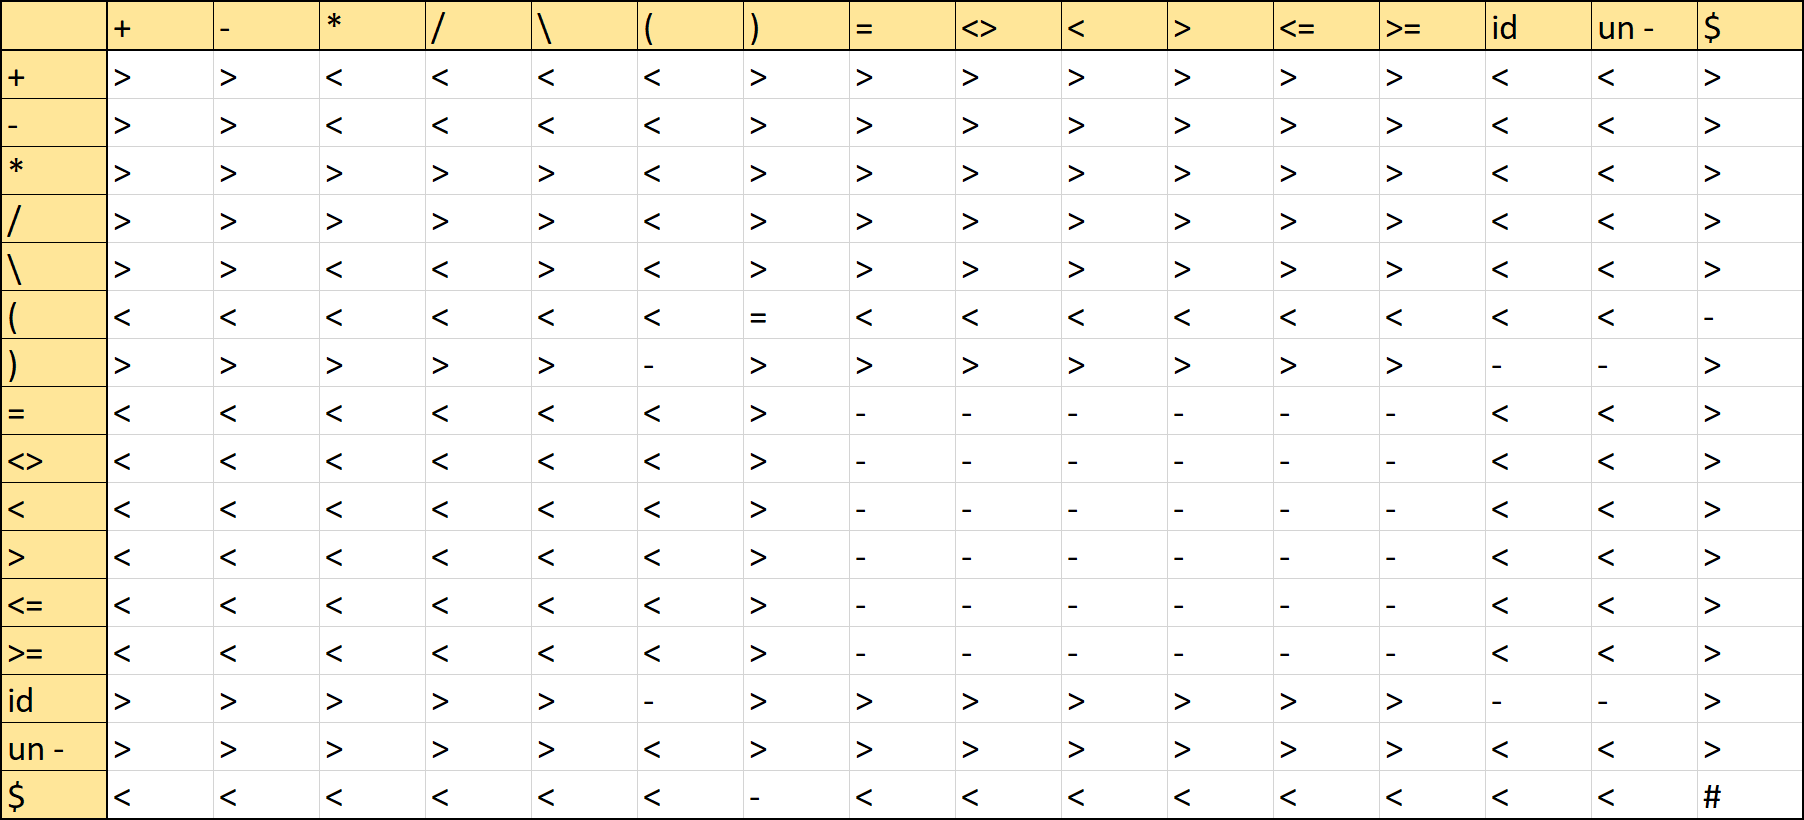
\includegraphics[width=17cm]{png/Precedencni_tabulka.png} 
	\caption{Precedenční tabulka}

\begin{figure}[H]
	
	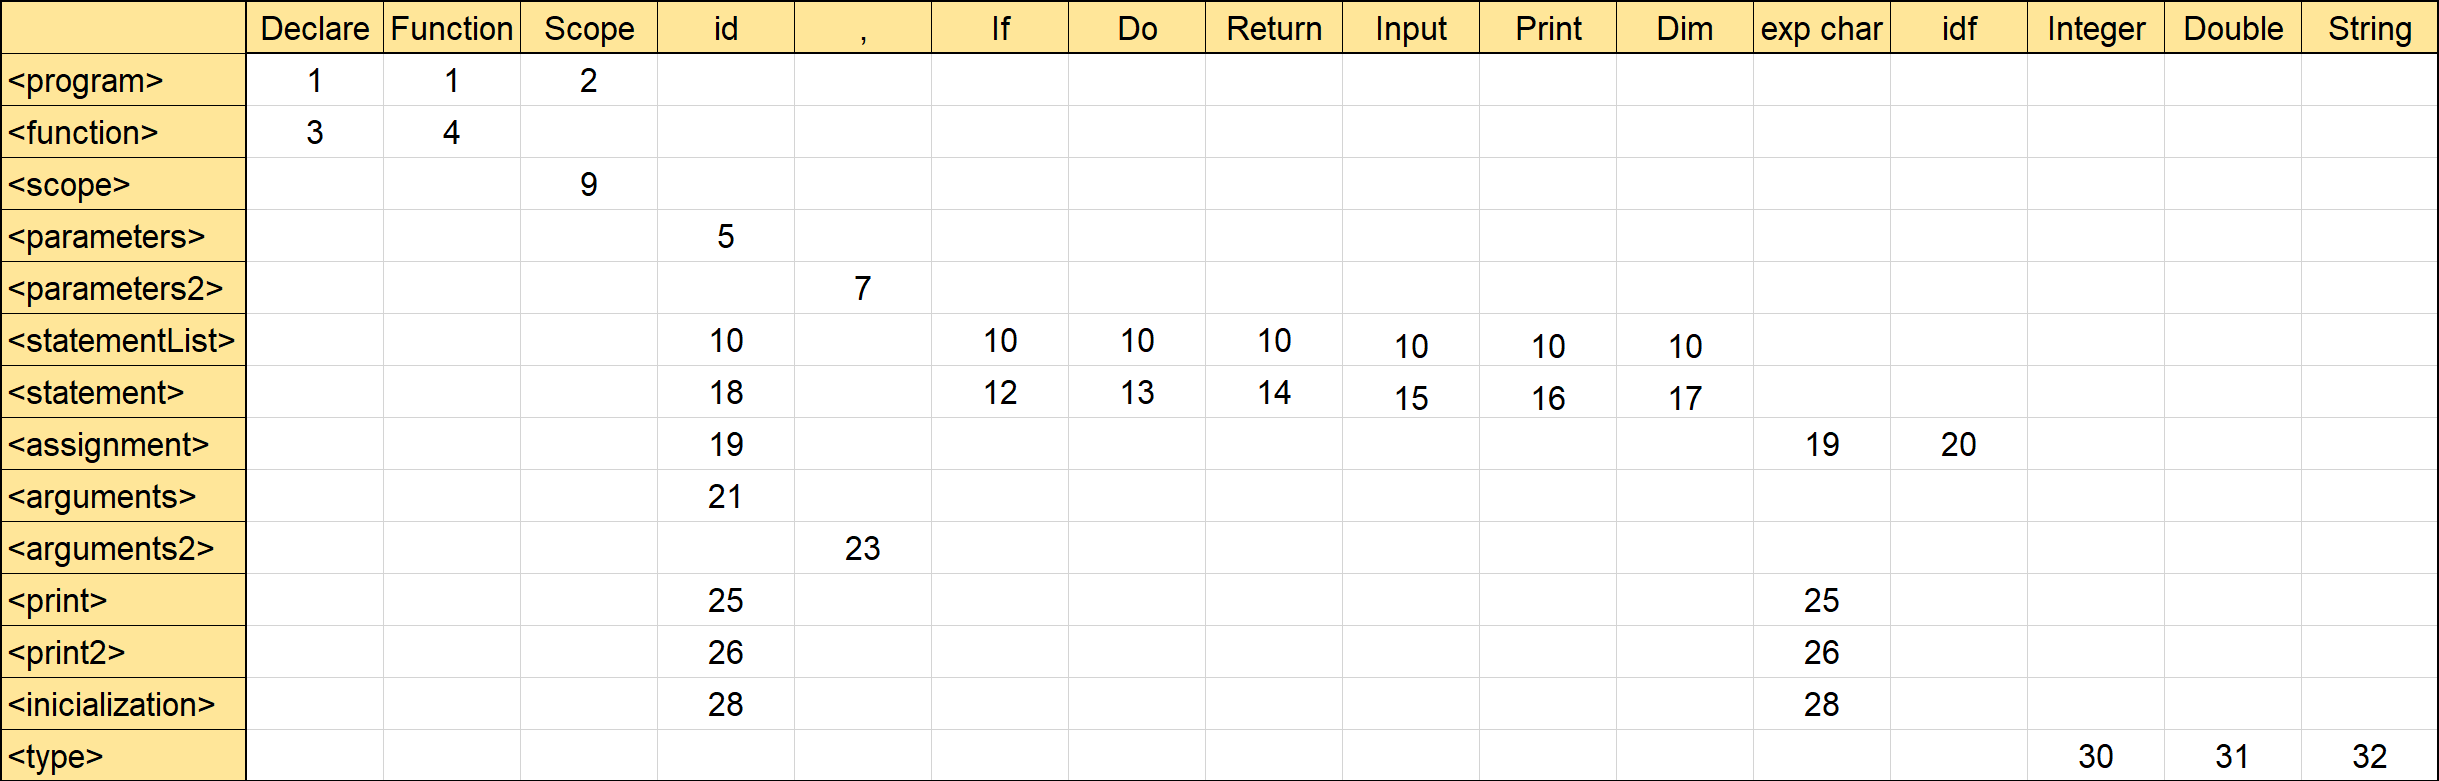
\includegraphics[width=17cm]{png/LL_Tabulka.png} 
	\caption{LL tabulka bez \epsilon přechodů (čísla v tabulce označují číslo gramatiky)}

\end{figure}

\end{figure}

\begin{figure}[H]
	
	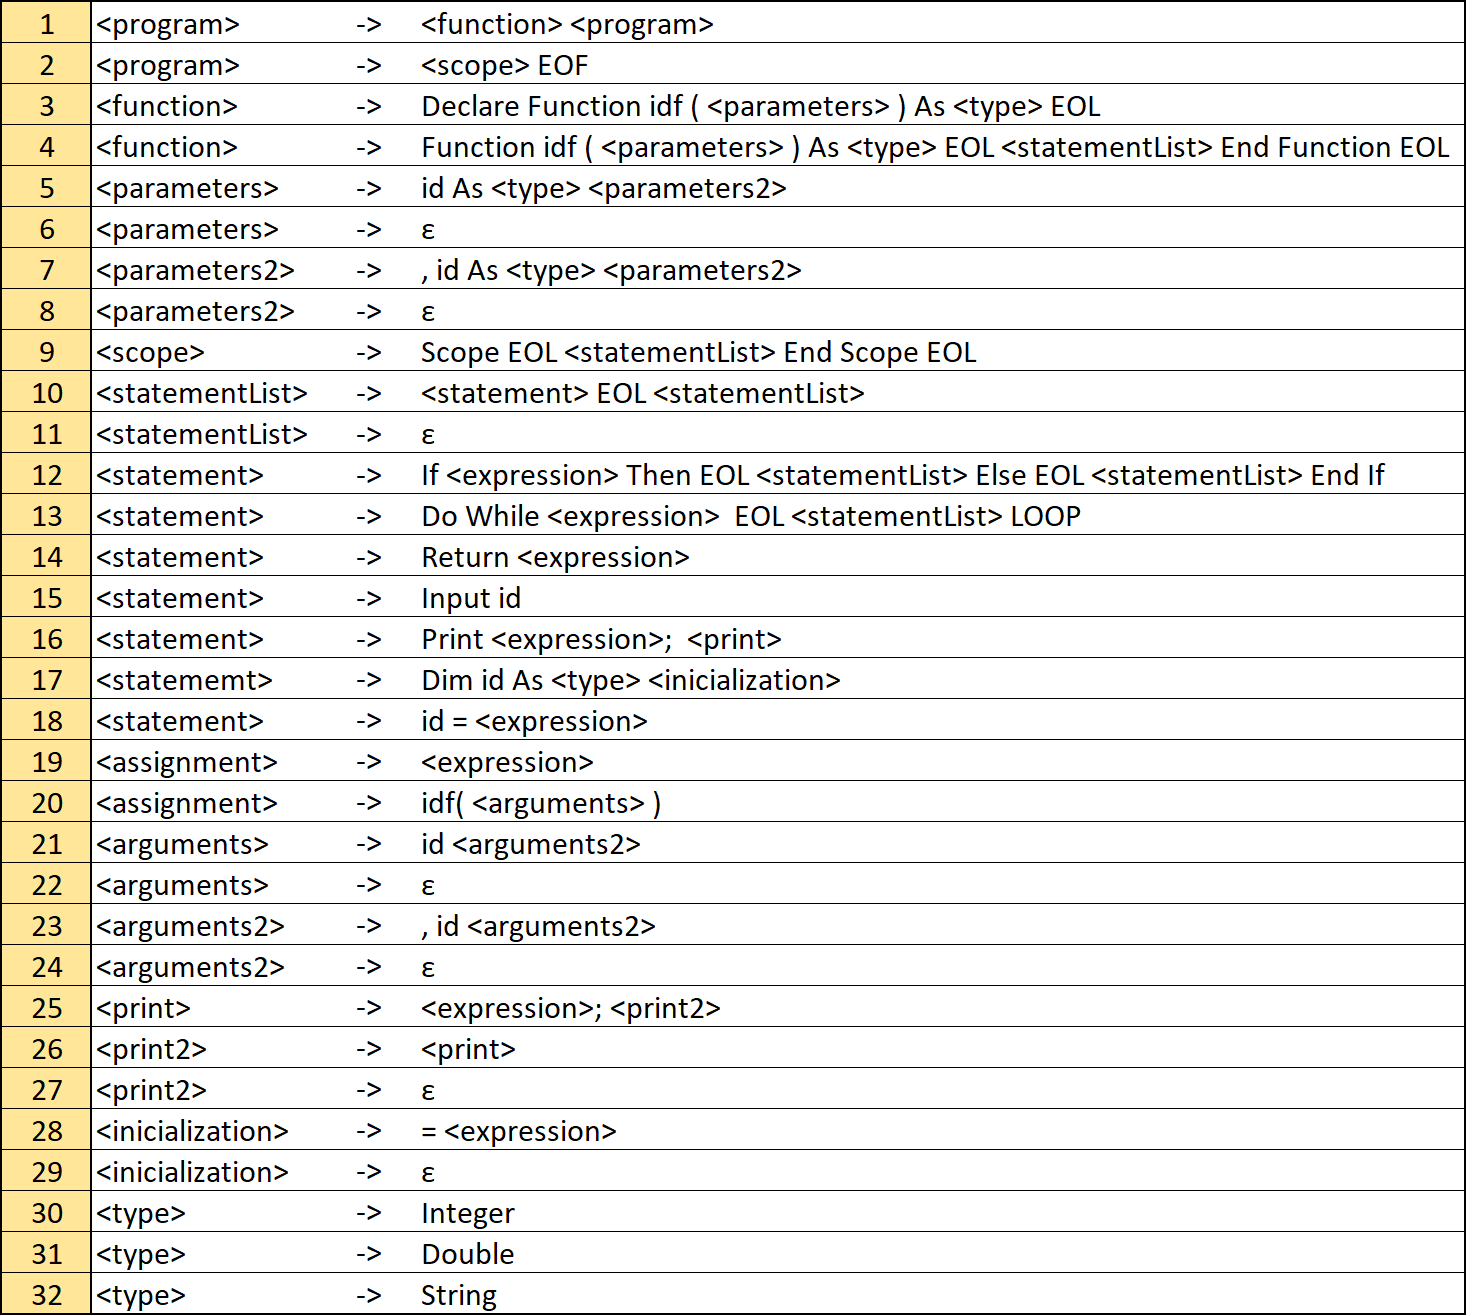
\includegraphics[width=17cm]{png/LL_Gramatika.png} 
	\caption{Tabulka LL gramatik}

\end{figure}


\section{Sémantická analýza}
Sémantickou analýzu jsme implementovali v~souboru \verb|parser.c|, kde probíhají všechny sémantické kontroly. Mezi hlavní kontroly patří redefinice proměnných, použití nedefinovaný proměnných, kompatibilita typů a počty argumentů ve funkcích, které byly realizovány tabulkou symbolů. 

Pro lepší orientaci v~kontextu definic a deklarací funkcí jsme si zavedli 3 módy, které slouží k~přesnému určení chyby (použití se nachází např. v~\verb|parser.c| ve funkci function() ). Módy měníme na základě přicházejících tokenů a hledání v~tabulce symbolů.

\begin{itemize}
\setlength\itemsep{0.3em}
\item \textbf{mód 0} -- jsme v~deklaraci funkce 
\item \textbf{mód 1} -- jsme v~definici funkce s~tím, že funkce je již deklarovaná 
\item \textbf{mód 2} -- definice je zároveň deklarací
\end{itemize}


\subsection{Funkce z pohledu sémantické analýzy}
void \textbf{function}() -- kontrola redefinice a redeklarace funkce s~vuyžitím námi zvolených módů

\noindent
void \textbf{parameters}(int \verb|mode|, \verb|htab_listitem *fce|) společně s funkcí \textbf{parameters2} -- kontrola počtu argumentů funkce a typy parametrů


\section{Tabulka symbolů}
Měli jsme za úkol implementovat tabulku symbolů pomocí rozptylovací tabulky. Vycházeli jsme z~přístupů probíraných v~předmětu IAL. Hashovací funkci jsme použili z~předmětu IJC, jelikož se nám zdála nejvhodnější pro projekt. 

\subsection{Struktura tabulky}

bool \verb|is_global| -- jestli se jedná o~globální (true) anebo lokální (false) tabulku

\noindent
unsigned int \verb|size_sym| -- velikost rozptylovací tabulky, kterou jsme zvolili na 769

\noindent
unsigned \verb|actual_number| -- aktuální počet položek  v~tabulce

\noindent
struct \verb|htab_listitem *symtab_item[]| -- ukazatel na pole seznamů \verb|htab_listitem|

\subsection{ADT seznam jako položka v tabulce symbolů}
bool \verb|is_defined| - příznak, jestli byla funkce nebo proměnná definovaná

\noindent
char \verb|*name| - název funkce/proměnné -- náš klíc podle kterého vkládáme/vyhledáváme

\noindent
\verb|Type_data| \verb|data_type| -- typ proměnné pro proměnnou, typ, který vrací funkce pro funkci

\noindent
unsigned int \verb|counter_params| - počet parametrů

\noindent
\verb|Tparam *params| -- seznam parametrů (počet \verb|counter_params|) typu TParam, což je struktura, která obsahuje název parametru, typ a ukazatel na další parametr

\noindent
\verb|TSymtable *local_table| - odkaz na lokální tabulku symbolů

\noindent
struct \verb|htab_listitem *next| - ukazatel na další prvek

\subsection{Funkce nad TS}

TSymtable *\textbf{symtabInit}(unsigned int \verb|size_symtable|) -- inicializuje tabulku a nastaví její velikost \\


\noindent
unsigned int \verb|hash_function|(const char *str) - hashovací funkce \\

\noindent
void \textbf{symtabClear}( TSymtable *table ) -- vyčistí celou tabulku a uvolní ji \\

\noindent
struct \verb|htab_listite|m *\textbf{symtabLookAdd}(TSymtable *symtable, char \verb|*token_data|) -- podívá se, jestli token se jménem \verb|token_data| ještě není v~tabulce a případně ho vloží do tabulky \\


\noindent
struct \verb|htab_listitem| *\textbf{symtabAddParam}(TSymtable *symtable, char \verb|*token_data|, \verb|Type_data| \\ \verb|type_param|, char \verb|*name_param|) -- přidá do tabulky 1 parametr se jménem \verb|name_param| a typem \verb|type_param| do záznamu v~seznamu s~klíčem \verb|token_data| \\


\noindent
struct \verb|htab_listitem| *\textbf{symtabAddType}(TSymtable *symtable, char \verb|*token_data|, \verb|Type_data| \\ \verb|type_variable|) -- přidá typ podle klíče \verb|token_data| \\


\noindent
struct \verb|htab_listitem| *\textbf{symtabFind}(TSymtable *table, const char *key) -- hledá klíč key a vrací ukazatel na strukturu \verb|htab_listitem|, v~případě nenalezení vrací NULL \\


\noindent
bool \textbf{isDefined} (TSymtable *table) -- prohledá celou tabulku, jestli všechny položku jsou definované tzn. mají nastaveno \verb|is_defined| = true \\



\section{Generování}
Generování tříadresného kódu jsme implementovali v~návaznosti na syntaktickou a sémantickou analýzu. Pro jednoduchost a rychlost implementace jsme využili možnost generování přímo v~rámci souborů \verb|parser.c| a \verb|expression.c|. Díky určitým vlastnostem jazyka (dopředné deklarace, scope až na konci zdrojového kódu atd\dots) generujeme při prvním průchodu společně s~analýzou. Řešili jsme různé problémy -- např. při rekurzivním volání funkcí nebo při použití vnořených cyklů - trvalo nám ponděkud delší dobu, než jsme si uvědomili vhodnost použití ADT zásobníku pro číslované návěští vnořených konstrukcí if a do while.

Pomocné datové struktury a funkce pro generování se vyskytují v~\verb|generator.c|. Pro ukládání instrukcí jsme si vybrali ADT lineárně vázaný seznam.


\section{Testování}
Testovali jsme každou vytvořenou část unit testy. Máme testy na lexikální analyzátor, testy na tabulku s~rozptýlenými položkami, testy na práci se zásobníkem a testy na práci se seznamem použitým pro generování. Pro celkové testování překladače jsme využili testy od spolužáků, kteří je měli dobře zpracované (podle těch testů jsme ladili syntax, sémantiku a generování). 

\section{Práce v~týmu}
První schůzka se uskutečnila v~úterý 26. 9. 2017 a od té doby jsme se pravidelně každé úterý scházeli. Na začátku jsme si zvolili komunikační kanály -- slack a facebook, zároveň jsme založili repozitář na githubu, kam jsme po celou dobu řešení projektu přidávali části kódu a určili jsme si tzv. code style, jelikož každý píše trochu jinak, a proto bylo vhodné si určit pravidla pro psaní kódu. Termíny jsme neměli pevně dané, proto na konci byl větší tlak na generování. To byl zřejmě největší náš problém. \\

\subsection{Rozdělení práce}

\subsubsection*{Alena Tesařová (xtesar36)}
\begin{itemize}
\setlength\itemsep{0.3em}
\item testy pro lexikální analyzátor\ (\verb|tests_lex.c|) 
\item testy pro hashovací tabulku\ (\verb|tests_symtable.c|)
\item testy pro zásobník\ (\verb|tests_stack.c|) 
\item implementace zásobník\ (\verb|stack.c, stack.h|) 
\item implementace hashovací tabulky\ (\verb|symtable.c, symtable.h|)
\item základní chybové výpisy\ (\verb|error.c, error.h|) 
\item Makefile
\end{itemize}

\subsubsection*{Jan Šorm (xsormj00)}
\begin{itemize}
\setlength\itemsep{0.3em}
\item syntaktická a sémantická analýza\ (\verb|parser.c, parser.h|) 
\item zpracování výrazů pomocí precedenční tabulky\ (\verb|expression.c|, \verb|expression.h|) 
\item LL tabulka, LL gramatika, precedenční tabulka
\item doplnění chybových výpisů (\verb|error.c, error.h|) 
\item část generování
\end{itemize}

\subsubsection*{Daniel Uhříček (xuhric00)}
\begin{itemize}
\setlength\itemsep{0.3em}
\item generování\ (\verb|parser.c|, \verb|expression.c|) 
\item implemetace jednosměrného seznamu pro ukládání výpisu generování\ (\verb|generator.c|, \verb|generator.h|) 
\item testy na generování\ (\verb|tests_generator.c|) 
\item \verb|main.c| 
\item Makefile
\end{itemize}

\subsubsection*{Peter Uhrín (xuhrin02)} 
\begin{itemize}
\setlength\itemsep{0.3em}
\item lexikální analýza\ (\verb|lex.c, lex.h, token.h|) 
\item konečný automat pro lexikální analyzátor
\end{itemize}


\section{Poznámky}
Velikost rozptylovací tabulky jsme zvolili 769, protože minimalizuje shlukování položek v~seznamu.
\begin{sloppypar}
\url{ http://www.orcca.on.ca/~yxie/courses/cs2210b-2011/htmls/extra/PlanetMath_%20goodhashtable.pdf }.
\end{sloppypar}


\section{Závěr}
Fungování interpretu odpovídá požadovanému zadání. V~prvním odevzdání se nám nepodařilo generovat kód, avšak v~druhém odevzdání se nám podařilo projekt vylepšit a získali jsme krásných 86 \%. I~když byl projekt časově velice náročný, získali jsme spoustu cenných zkoušeností, které se určitě budou hodit do dalších let. Tímto děkuji všem členům, protože odvedli všichni skvělou práci.


\end{document}
